\documentclass{report}
\usepackage{graphicx}
\usepackage{sidecap}
\usepackage{fancyhdr}
\usepackage{lscape}
\usepackage[absolute]{textpos}
\usepackage{SIunits}
\usepackage{sistyle}
\usepackage{amsmath}

\makeatletter
\def\maketitle{%
  \null
  \thispagestyle{empty}%
  \vfill
  \begin{center}\leavevmode
    \normalfont
    {\LARGE \@title\par}%
    \vskip 1cm
    {\Large \@author\par}%
    \vskip 1cm
    {\Large \@date\par}%
  \end{center}%
  \vfill
  \null
  \newpage
  }
\makeatother
\author{Groupe : Mattens Simon, Dom Eduardo\\ BAB2 Sciences Informatiques}
\title{Rapport : circuits RC et RL}


\begin{document}
\maketitle

\section*{1 Introduction}
\hspace*{0.5cm}

\'Etude de la charge et de la d\'echarge d'un condensateur C \`a travers une r\'esistance R visualis\'ee au moyen du programme informatique LabView. V\'erification de la loi exp\'erimentale de la loi de l'association de capacit\'es.

\section*{2 R\'esum\'e th\'eorique}
\subsection*{2.1 Les condensateurs}
\hspace*{0.5cm}
La capacit\'e \'equivalente pour un montage en s\'erie des condensateurs est donn\'ee par:

\begin{equation}
   \frac{1}{C_{eq}} =  \sum{\frac{1}{C_{i}}}
\end{equation}

Pour un montage en parall\`ele des condensateurs, la formule est:

\begin{equation}
    C_{eq} =\sum{C_{i}}
\end{equation}

La charge d'un condensateur \`a travers une r\'esistance est donn\'ee par:
\begin{equation}
    Q(t) = Q_{0}(1-e^{\frac{-t}{\tau}})
\end{equation}

Quant \`a la d\'echarge, la formule est la suivante :
\begin{equation}
    Q(t) = Q_{0}e^{\frac{-t}{\tau}}
\end{equation}

L'unit\'e des capacit\'es est exprim\'e en Farad. Un condensateur charg\'e ne laisse pas passer le courant continu. En effet, il existe un isolant entre les armatures.

Les capacit\'es sont d\'efinies par cette relation:
\begin{equation}
    Q = C\cdot U
\end{equation}

\subsection*{2.2 La loi d'Ohm}
\hspace*{0.5cm}
La r\'esistance \'electrique d\'etermine l'intensit\'e du courant traversant le conducteur en fonction de la valeur de la tension appliqu\'ee \`a ses bornes.

\begin{equation}
    U = R \cdot I
\end{equation}


\section*{3 Dispositif exp\'erimental}
\subsection*{3.1 Mat\'eriel utilis\'e}
\begin{itemize}
\item R\'esistances et condensateurs de type \'electrolytique  ainsi qu'une plaque de r\'ealisation de circuits.

\item Un g\'en\'erateur de tension continue (de 0 \`a 30 V) r\'eglable via les deux potentiom\`etres : COARSE et FINE.

\item Un multim\`etre de marque Keithley de type 2010 utilis\'e en voltm\`etre. Il est \'equip\'e d'une sortie IEEE.

\item PC d'acquisition pour utiliser le logiciel LabView. Le PC est reli\'e au voltm\`etre et \`a la carte d'acquisition GPIB au moyen d'un c\^able de type GPIB.

\item Un g\'en\'erateur de tension alternative de forme carr\'ee. Celui-ci permet de stabiliser le comportement du circuit.

\item Un oscilloscope.
\end{itemize}

\subsection*{3.2 Conditions de mesure pour le VI}
\hspace*{0.5cm}
La pr\'ecision de lecture a \'et\'e fix\'ee \`a digits 2 (=5 1/2 digits de r\'esolution. Le wait time - le temps entre chaque mesure - est de 5 secondes. Le pourcentage de charge totale est de 0.97 et le pourcentage de d\'echarge (r\'eglant les arr\^et mesure) est \`a 0.03. La tension appliqu\'ee est de 10V.
\pagebreak
\section*{4 Prise des mesures \& r\'esultats}
\subsection*{4.1 Charge d'un condensateur \`a travers une r\'esistance}
\hspace*{0.5cm}
\begin{figure}[ht!]
\centering
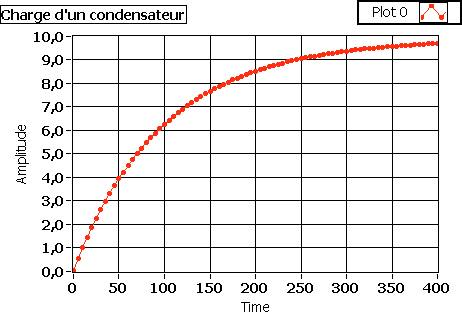
\includegraphics[width=90mm]{chargeCond.jpg}
\label{overflow}
\end{figure}
\\
\hspace*{0.5cm}
Nous constatons que le condensateur charge plus vite au d\'ebut de la manipulation qu'\`a la fin. De plus la charge du condensateur tend vers 10V sans l'atteindre. Il a fallu 400 secondes pour s'approcher sensiblement du voltage maximum.
\pagebreak
\subsection*{4.2 D\'echarge d'un condensateur \`a travers une r\'esistance}
\begin{figure}[ht!]
\centering
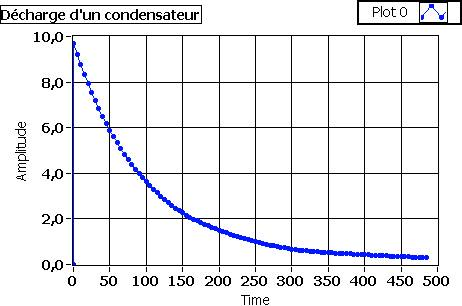
\includegraphics[width=90mm]{dechargeCond.jpg}
\label{overflow}
\end{figure}
\hspace*{0.5cm}
Nous constatons que le condensateur se d\'echarge plus vite au d\'ebut de la manipulation qu'\`a la fin. De plus le condensateur ne se d\'echarge pas compl\`etement. Il a fallu approximativement 500 secondes pour que le condensateur se d\'echarge totalement.
\pagebreak
\section*{5. Analyse des r\'esultats}
\begin{figure}[ht!]
\centering
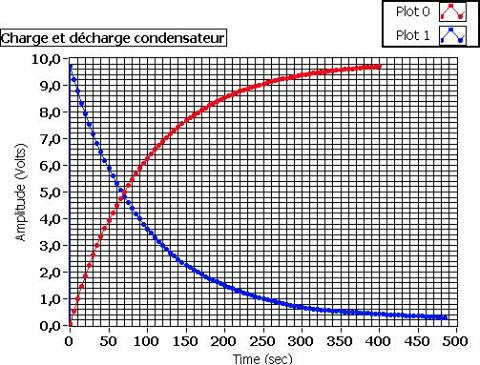
\includegraphics[width=90mm]{analyse2.jpg}
\label{overflow}
\end{figure}
\begin{figure}[ht!]
\centering
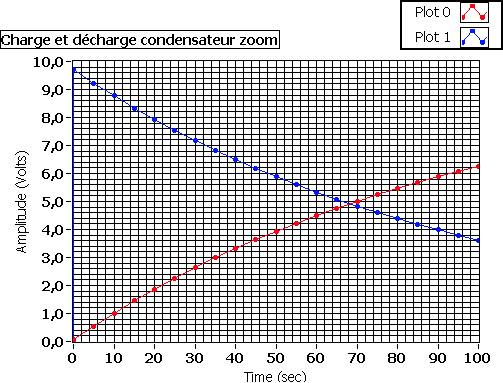
\includegraphics[width=90mm]{analyse1.jpg}
\label{overflow}
\end{figure}
\hspace*{0.5cm}
Les courbes s'intersectent \`a la demi-vie $\tau$ de la charge et de la d\'echarge du condensateur. C'est le temps n\'ecessaire pour que la tension aux bornes du condensateur atteigne la moiti\'e de sa valeur maximale.
\subsection*{5.1 Analyse dimensionnelle de la constante de temps $\tau$ }
V\'erifions que $\tau$ = RC a bien des unit\'es de temps.
\\
On a donc:
   $$[\tau] = 1\Omega \cdot 1F$$
Par la loi d'Ohm, on a alors:
   $$[\tau] = \frac{1V \cdot 1F}{1A}$$
Or, on sait que:
   $$1F = \frac{1s \cdot 1A}{1V}$$
Donc,
   $$[\tau] = \frac{1V \cdot 1s \cdot 1A}{1A \cdot 1V}$$
  $$\Leftrightarrow [\tau] = 1s$$
L'unit\'e internationale du temps est la seconde. $\tau$ a bien des unit\'es de temps.  

\subsection*{5.2 D\'eduction de la constante de temps via le trac\'e de la tangente de la courbe exponentielle.}
\hspace*{0.5cm}

\begin{figure}[ht!]
\centering
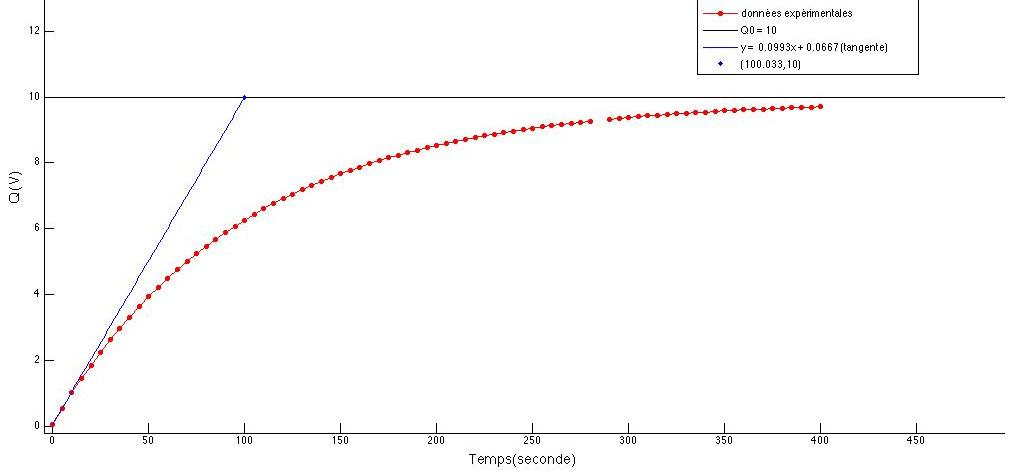
\includegraphics[width=140mm]{3-1graph243.jpg}
\caption{Tangente \`a la courbe exponentielle au temps t = 0 s'intersectant avec la droite horyzontal Q = Q0.}
\label{overflow}
\end{figure}
\pagebreak
Le point d'intersection entre la tangente \`a la courbe exponentielle au t = 0 et la droite horyzontale Q = Q0 a les coordonn\'ees suivantes:
\begin{equation}
   P = (100,033;10)
\end{equation}
Nous en d\'eduisons que, exp\'erimentalement, nous avons une constante de temps $\tau$ = 100,033 secondes.
\subsection*{5.3 Justification math\'ematique du proc\'ed\'e de d\'etermination de $\tau$.}
\hspace*{0.5cm}
Pour savoir le point d'intersection entre la tangente et la droite Q = Q0, on doit savoir l'\'equation de cette tangente.
Pour ce faire, nous devons approximer la courbe exponentielle au moyen d'un d\'evelloppement de Taylor d'ordre 6 (calcul\'e avec un logiciel) :
\begin{equation}
   P(x) = -3^{(-15)} \cdot x^6 + 6^{(-12)} \cdot x^5 - 4^{(-09)}\cdot x^4 + 2^{(-06)}\cdot x^3 - 0.0005\cdot x^2 + 0.0993\cdot x + 0.0667
\end{equation}
De par ce d\'evelloppement de Taylor, nous savons l'\'equation de la tangente:
\begin{equation}
   T(x) = -0.0993\cdot x + 0.0667
\end{equation}
On peut donc maintenant calculer le point d'intersection entre les deux droites :
\[
\left\{
\begin{array}{r c l}
y &=& 10\\
y &=& 0.0993\cdot x + 0.0667 (tangente)\\
\end{array}
\right.
\]
On obtient ainsi le point P :
\begin{equation}
   P = (100,033;10)
\end{equation}

\subsection*{5.4 Calcul th\'eorique de $\tau$ et comparaison avec la valeur mesur\'ee.}
\hspace*{0.5cm}
Pour calculer la valeur de $\tau$ th\'eoriquement, nous utilisons la formule ci-dessous:

\begin{equation}
    \tau = R \cdot C
\end{equation}

Pour r\'ealiser ce tp, nous avons utilis\'e une r\'esistance de $12\cdot 10^{5} \ohm$  et un condensateur de $68\micro F$.
\\
On obtient:
\begin{equation}
    \tau = 12\cdot 10^{5} \cdot 68\cdot 10^{-6}
\end{equation}

\begin{equation}
    \Leftrightarrow \tau = 81,6 \text{ secondes}
\end{equation}

\pagebreak
\subsection*{5.4 Circuit \`a constante de temps rapide}
\hspace*{0.5cm}
Apr\`es avoir r\'egl\'e la fr\'equence \`a 1 kHz et une forme de signal carr\'ee sur le g\'en\'erateur de signaux(GS) en tension alternative, nous avons visualis\'e cette tension sur l'oscilloscope.
\begin{figure}[ht!]
\centering
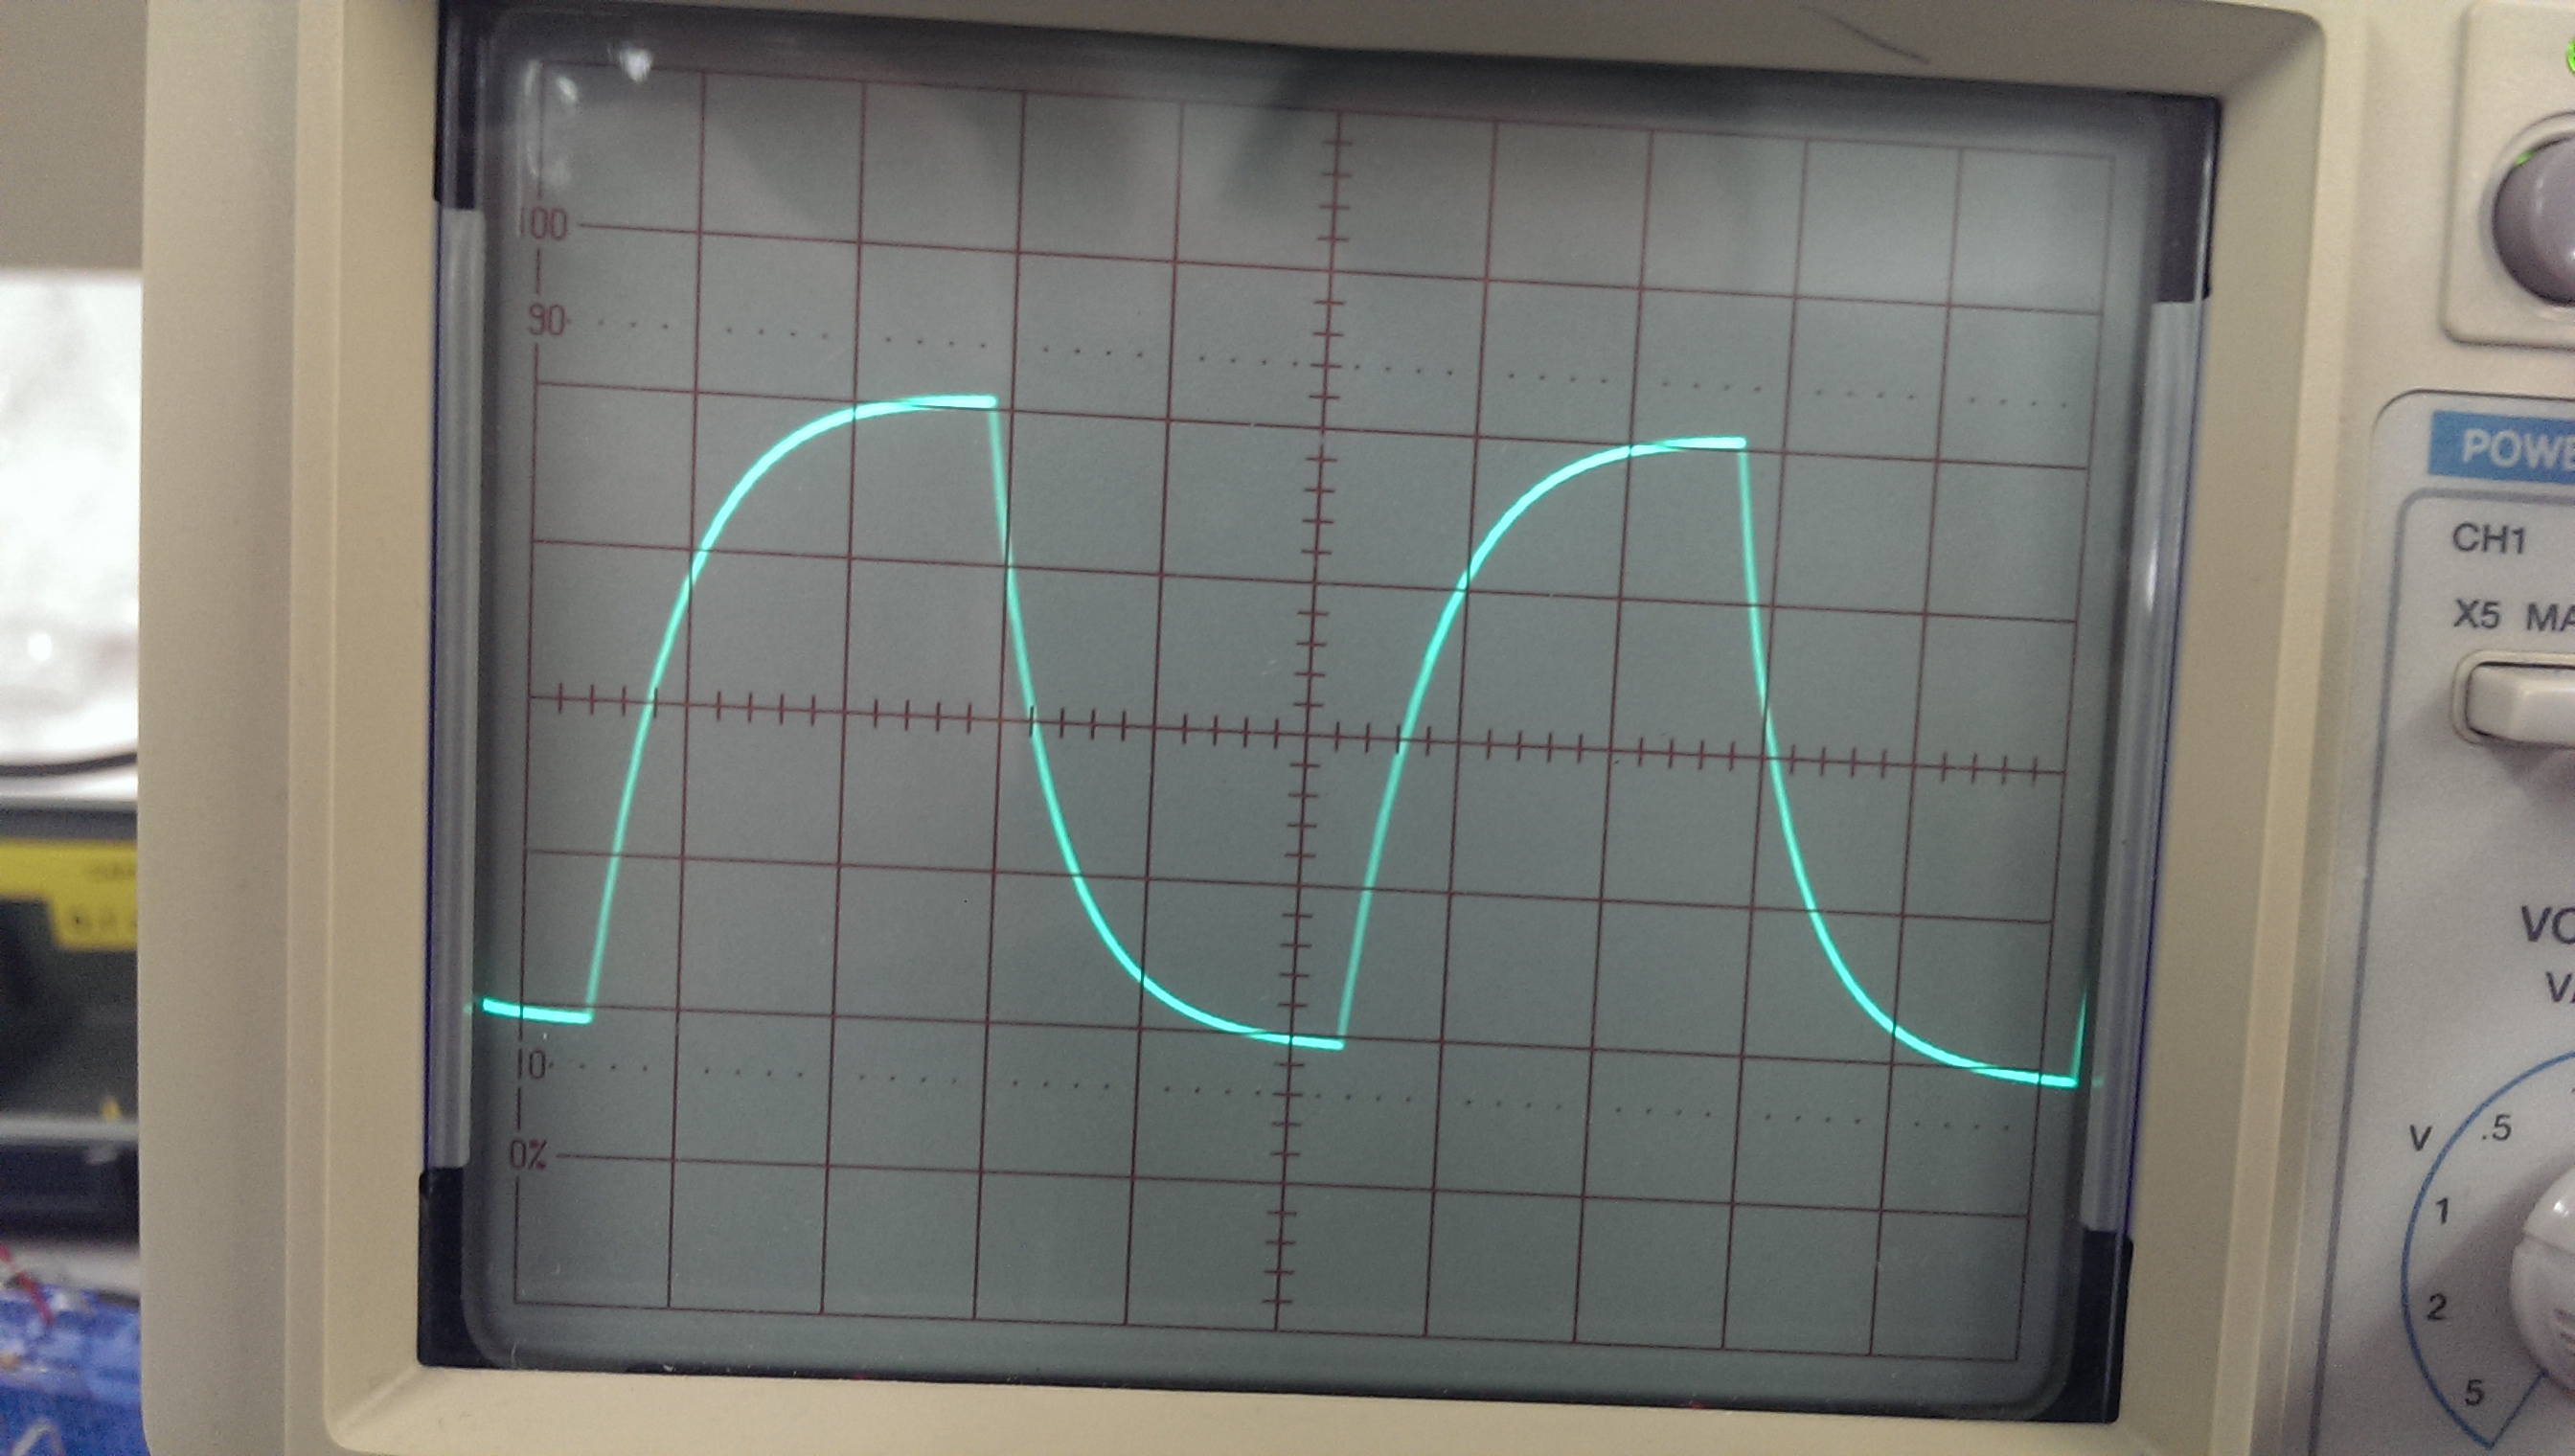
\includegraphics[width=90mm]{E244img1.jpg}
\caption{Tension visualis\'e.}
\label{overflow}
\end{figure}
L'amplitude est de 2 Volts et la p\'eriode de 0,5 seconde.

Nous avons ensuite branch\'e cette tension aux bornes du circuit RC. Le signal visualis\'e sur l'oscilloscope est ci-dessous.
\begin{figure}[ht!]
\centering
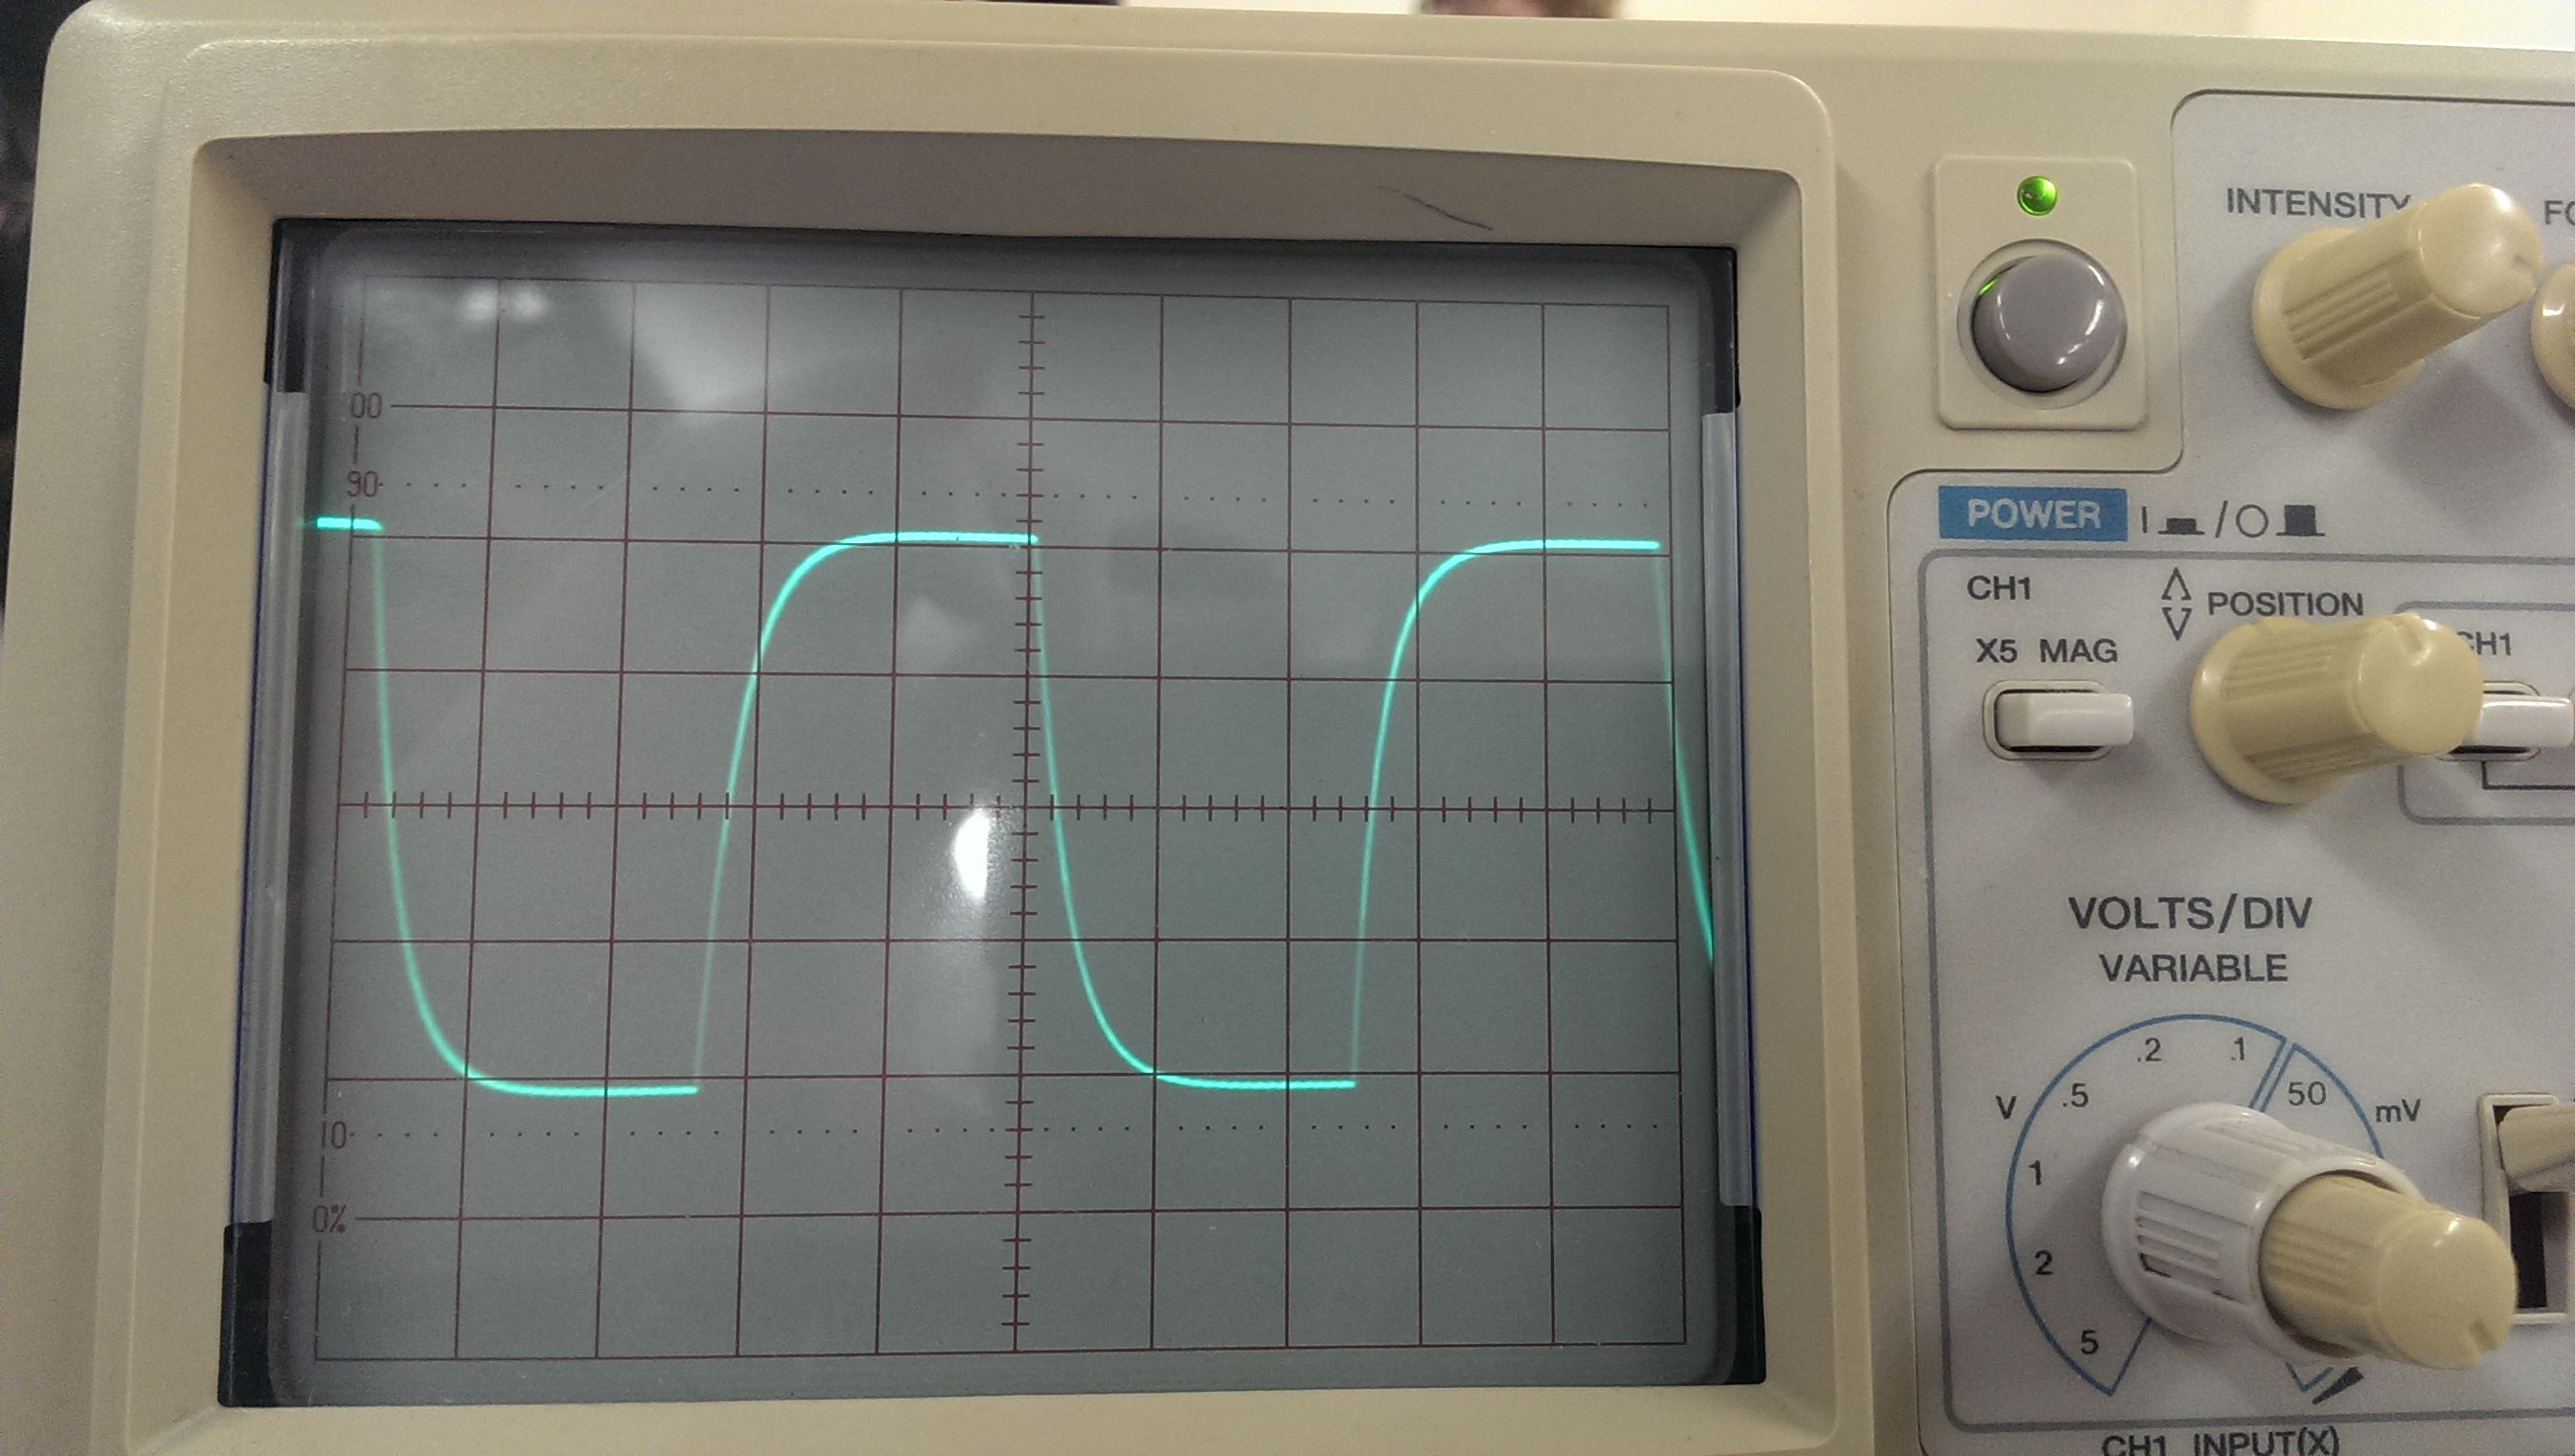
\includegraphics[width=90mm]{E244img2.jpg}
\caption{Tension visualis\'e.}
\label{overflow}
\end{figure}
\\
L'amplitude est toujours de 2 Volts et la p\'eriode est de 1 seconde.
Ensuite, nous avons calcul\'e exp\'erimentalement la demi-vie:
\begin{equation}
   T_{1/2} = \frac{0,3}{5}
\end{equation}
\pagebreak
\\
On peut maintenant calculer $\tau$:
\begin{equation}
   \tau = \frac{T_{1/2}}{ln2}
\end{equation}
\begin{equation}
   \Leftrightarrow \tau = \frac{0,3}{5 \cdot ln2} 
\end{equation}

\begin{equation}
   \Leftrightarrow \tau = 0.08656170245 \text{ seconde} 
\end{equation}
Valeur th\'eorique de $\tau$ : 0.001 seconde.
\\
Nous constatons que la valeur th\'eorique est plus petite que la valeur exp\'erimentale. D\`es lors, on doit tenir compte de la r\'esistance interne du g\'en\'erateur de signaux.
Pour calculer cette r\'esistance interne, nous savons que :
\begin{equation}
   R = \frac{\tau}{C} 
\end{equation}
\begin{equation}
  \Leftrightarrow R = \frac{0.08656170245}{0,1 \cdot 10^{-6}} 
\end{equation}
\begin{equation}
  \Leftrightarrow R = 865617.0245 \ohm
\end{equation}

\subsection*{5.5 V\'erification de la loi d'association des capacit\'es}
\subsubsection*{5.5.1 Capacit\'es mont\'ees en s\'erie}
\hspace*{0.5cm}
Nous avons remplac\'e la capacit\'e par 2 capacit\'es en s\'erie. Nous avons observer la d\'echarge. Nous avons \'egalement mesur\'e la demi-vie.
\begin{equation}
   T_{1/2} = \frac{0,2}{5}
\end{equation}

Comme les deux capacit\'es de 0,1\micro F sont mont\'ees en s\'erie, nous pouvons calculer th\'eoriquement C equivalent:

\begin{equation}
   \frac{1}{C_{eq}} =  \frac{1}{C_{1}}+\frac{1}{C_{2}}
\end{equation}

\begin{equation}
   \Leftrightarrow C_{eq} =  (\frac{1}{0,1 \cdot 10^{-6}}+\frac{1}{0,1 \cdot 10^{-6}})^{-1}
\end{equation}

\begin{equation}
   \Leftrightarrow C_{eq} = 5 \cdot 10^{-8} F
\end{equation}
\begin{equation}
   \Leftrightarrow C_{eq} = 0,05 \micro F
\end{equation}
\pagebreak
\\
Calculons maintenant C \'equivalent avec les valeurs empiriques.
\begin{equation}
    C_{eq} = \frac{\tau}{R}
\end{equation}
\begin{equation}
    \Leftrightarrow C_{eq} = \frac{\frac{T_{1/2}}{ln(2)}}{R}
\end{equation}
\begin{equation}
    \Leftrightarrow C_{eq} = \frac{0,2}{5 \cdot ln(2) \cdot R}
\end{equation}
\begin{equation}
    \Leftrightarrow C_{eq} = \frac{0,2}{5 \cdot ln(2) \cdot 865617.0245}
\end{equation}
\begin{equation}
    \Leftrightarrow C_{eq} = 6.66666686\cdot 10^{-8}
\end{equation}
\begin{equation}
    \Leftrightarrow C_{eq} = 0.066 \micro F
\end{equation}
Nous constatons que la diff\'erence de valeur entre C \'equivalent calcul\'e avec les valeurs empiriques et l'autre sont sensiblement proches. En effet, il n'y a que 0,016 \micro F de diff\'erence.
\subsection*{7.2 Capacit\'es mont\'ees en parall\`eles}
\hspace*{0.5cm}
Nous avons remplac\'e la capacit\'e par 2 capacit\'es en parall\`eles. Nous avons observer la d\'echarge. Nous avons \'egalement mesur\'e la demi-vie.
\begin{equation}
   T_{1/2} = \frac{0,6}{5}
\end{equation}
Comme les deux capacit\'es de 0,1\micro F sont mont\'ees en parall\`eles, nous pouvons calculer th\'eoriquement C equivalent:
\begin{equation}
    C_{eq} = C_1 + C_2
\end{equation}
\begin{equation}
    C_{eq} = 0,1 \cdot 10^{-6} +  0,1 \cdot 10^{-6}
\end{equation}
\begin{equation}
    C_{eq} = 2 \cdot 10^{-7}
\end{equation}
\begin{equation}
    C_{eq} = 0,2 \micro F
\end{equation}

Calculons maintenant C \'equivalent avec les valeurs empiriques.
\begin{equation}
    C_{eq} = \frac{\tau}{R}
\end{equation}
\begin{equation}
    \Leftrightarrow C_{eq} = \frac{\frac{T_{1/2}}{ln(2)}}{R}
\end{equation}
\begin{equation}
    \Leftrightarrow C_{eq} = \frac{0,6}{5 \cdot ln(2) \cdot R}
\end{equation}
\begin{equation}
    \Leftrightarrow C_{eq} = \frac{0,6}{5 \cdot ln(2) \cdot 865617.0245}
\end{equation}
\begin{equation}
    \Leftrightarrow C_{eq} = 2 \cdot 10^{-7}
\end{equation}
\begin{equation}
    \Leftrightarrow C_{eq} = 0,2 \micro F
\end{equation}
On constate que la valeur de C calcul\'e empiriquement est \'egale \`a la valeur de C calcul\'e th\'eoriquement.

\section*{6 Conclusion}
\hspace*{0.5cm}
Nous avons \'etudi\'e la charge et la d\'echarge exponentielle d'un condensateur C \`a travers une r\'esistance R visualis\'ee au moyen du programme LabView. On a aussi v\'erifi\'e la loi exp\'erimentale de la loi d'association de capacit\'es en s\'erie et en parall\`ele.\\

Tous nos r\'esultats concordaient avec ce que pr\'evoyait la th\'eorie.

\end{document}